\chapter{Выбор признаков в задаче декодирования сигналов}
\label{ch:qpfs}

Задача выбора признаков заключается в поиске оптимального подмножества~$\cA \subset \{ 1, \dots, n \}$ индексов признаков среди всех возможных $2^n - 1$ вариантов. 
Существует взаимооднозначное отображение между подмножеством $\cA$ и булевым вектором~$\ba \in \{0, 1\}^n$, компоненты которого указывают, выбран ли признак. 
Для нахождения оптимального вектора~$\ba$ введем функцию ошибки выбора признаков~$S(\ba, \bX, \bY)$. 
Проблема выбора признаков принимает вид:
\begin{equation}
	\ba = \argmin_{\ba' \in \{0, 1\}^n} S(\ba', \bX, \bY).
	\label{ch3:eq:feature_selection}
\end{equation}
Целью выбора признаков является построение функции~$S (\ba, \bX, \bY)$. Конкретные примеры данной функции для рассматриваемых методов выбора признаков приведены ниже и обобщены в таблице~\ref{ch3:tbl:summary}.

Задача~\eqref{ch3:eq:feature_selection} имеет дискретную область определения~$\{0, 1\}^n$. Для решения данной задачи применяется релаксация задачи~\eqref{ch3:eq:feature_selection} к непрерывной области определения~$[0, 1]^n$. Релаксированная задача выбора признаков имеет следующий вид:
\begin{equation}
	\bz = \argmin_{\bz' \in [0, 1]^n} S(\bz', \bX, \bY).
	\label{ch3:eq:relaxed_feature_selection}
\end{equation}

Здесь компоненты вектора~$\bz$~--- значения нормированных коэффициентов значимости признаков.
Сначала решается задача~\eqref{ch3:eq:relaxed_feature_selection}, для получения вектора значимостей~$\bz$. 
Затем решение~\eqref{ch3:eq:feature_selection} восстанавливается с помощью отсечения по порогу следующим образом:
\begin{equation}
	\ba = [a_j]_{j=1}^n, \quad 
	a_j = \begin{cases}
		1, & z_j > \tau; \\
		0, & \text{в противном случае}.
	\end{cases}
	\label{ch3:eq:feature_threshold}
\end{equation}
$\tau$~--- гиперпараметр, который может быть подобран вручную или выбран с помощью кросс-валидации. 

Как только решение~$\ba$ задачи~\eqref{ch3:eq:feature_selection} получено, задача~\eqref{ch1:eq:l2_loss_function} принимает вид:
\begin{equation*}
	\mathcal{L}(\bTheta_{\cA}, \bX_{\cA}, \bY) = {\left\| \mathbf{Y} - \bX_{\cA}\bTheta_{\cA} \right\| }_2^2 \rightarrow\min_{\bTheta_{\cA}},
\end{equation*}
где индекс~$\cA$ обозначает подматрицу со столбцами, индексы которых содержатся в~$\cA$.

%%%%%%%%%%%%%%%%%%%%%%%%%%%%%%%%%%%%%%%%%%%%%%%%
\section{Выбор признаков с помощью квадратичного программирования}
\label{sec:ch3:qpfs_feature_selection}
%%%%%%%%%%%%%%%%%%%%%%%%%%%%%%%%%%%%%%%%%%%%%%%%

Если между столбцами матрицы исходных объектов~$\bX$ существует линейная зависимость, то решение задачи линейной регрессии
\begin{equation}
	\| \bnu - \bX \btheta\|_2^2 \rightarrow\min_{\btheta \in \bbR^{n}}.
	\label{ch3:eq:linear_regression}
\end{equation}
оказывается неустойчивым. 
Методы выбора признаков находят подмножество~$ \cA \in \{1, \dots, n\}$ оптимальных столбцов матрицы~$\bX$. 

Метод QPFS~\cite{rodriguez2010quadratic} выбирает некоррелированные признаки, релевантные целевому вектору~$\bnu$.
Чтобы формализовать этот подход, введем две функции: $\text{Sim}(\bX)$ и $\text{Rel}(\bX, \bnu)$. 
$\text{Sim}(\bX)$ контролирует избыточность между признаками, $\text{Rel}(\bX, \bnu)$ содержит релевантности между каждым признаком и целевым вектором. 
Мы хотим минимизировать функцию Sim и максимизировать Rel одновременно.

QPFS предлагает явный способ построения функций Sim и Rel. 
Метод минимизирует следующую функцию ошибки
\begin{equation}
	\underbrace{\bz^{\T} \bQ \bz}_{\text{Sim}} - \alpha \cdot \underbrace{\vphantom{()} \mathbf{b}^{\T} \bz}_{\text{Rel}} \rightarrow \min_{\substack{\bz \in \bbR^n_+ \\ \|\bz\|_1=1}}.
	\label{ch3:eq:qpfs_problem}
\end{equation}
Элементы матрицы парных взаимодействий~$\bQ \in \bbR^{n \times n}$ содержат коэффициенты попарного сходства между признаками. 
Вектор релевантностей признаков~$\mathbf{b} \in \bbR^n$ выражает сходство между каждым признаком и целевым вектором~$\bnu$.
Нормированный вектор~$\bz$ отражает значимость каждого признака. 
Функция ошибки~\eqref{ch3:eq:qpfs_problem} штрафует зависимые признаки функцией Sim и штрафует признаки, не релевантные к целевой переменной функцией Rel. 
Параметр~$\alpha$ позволяет контролировать компромисс между Sim и Rel.
Авторы оригинальной статьи QPFS~\cite{rodriguez2010quadratic} предложили способ выбора~$\alpha$, чтобы уравновесить вклад членов $\text{Sim}(\bX)$ и $\text{Rel}(\bX, \bnu)$

\begin{equation*}
	\alpha = \frac{\overline{\bQ}}{\overline{\bQ} + \overline{\bb}}, \quad \text{где}\,\,\overline{\bQ} = \text{mean} (\bQ), \,\,\, \overline{\bb}= \text{mean} (\bb).
\end{equation*}
Чтобы выделить оптимальное подмножество признаков, применяется отсечение по порогу~\eqref{ch3:eq:feature_threshold}.

Для измерения сходства используется выборочный коэффициент корреляции Пирсона между парами признаков для функции Sim, и между признаками и целевым вектором для функции Rel:
\begin{equation}
	\bQ = \left[|\text{corr}(\bchi_i, \bchi_j)|\right]_{i,j=1}^n, \quad \bb = \left[|\text{corr}(\bchi_i, \bnu)|\right]_{i=1}^n.
	\label{ch3:eq:qpfs_1d_qb}
\end{equation}
Здесь
\begin{equation*}
\text{corr}(\bchi, \bnu) = \frac{\sum_{i=1}^m(\bchi_i - \overline{\bchi})( \bnu_i - \overline{\bnu})}{\sqrt{\sum_{i=1}^m(\bchi_i - \overline{\bchi})^2\sum_{i=1}^m(\bnu_i - \overline{\bnu})^2}}.
\end{equation*}
Другие способы определения $\bQ$ и $\bb$ рассматриваются в~\cite{katrutsa2017comprehensive}. 
В работе~\cite{katrutsa2017comprehensive} показано, что метод QPFS превосходит многие существующие методы выбора признаков на различных внешних критериях качества.

Задача~\eqref{ch3:eq:qpfs_problem} является выпуклой, если матрица~$\bQ$ является неотрицательно определенной. В общем случае это не всегда верно. 
Чтобы удовлетворить этому условию спектр матрицы~$\bQ$ смещается, и матрица~$\bQ$ заменяется на $\bQ - \lambda_{\text{min}} \mathbf{I}$, где $\lambda_{\text{min}} $ является минимальным собственным значением~$\bQ$.

%%%%%%%%%%%%%%%%%%%%%%%%%%%%%%%%%%%%%%%%%%%%%%%%
\section{Методы выбора признаков для случая векторной целевой переменной}
\label{sec:ch3:mqpfs_feature_selection}
%%%%%%%%%%%%%%%%%%%%%%%%%%%%%%%%%%%%%%%%%%%%%%%%

В данном разделе описаны предлагаемые методы выбора признаков для случая векторной целевой переменной.
В этом случае компоненты целевой переменной могут коррелировать между собой. 
Предлагаются методы, учитывающие зависимости как в исходном, так и в целевом пространствах.

\textbf{Агрегация релевантностей целевых векторов.}
В работе~\cite{motrenko2018multi}, чтобы применить метод QPFS к векторному случаю ($r > 1$), релевантности признаков агрегируются по всем $r$ компонентам целевой переменной. 
Член $\text{Sim}(\bX)$ остаётся без изменений, матрица парных взаимодействий~$\bQ$ определяется как~\eqref{ch3:eq:qpfs_1d_qb}. 
Вектор релевантностей $\bb$ агрегируется по всем компонентам целевой переменной и определяется как
\begin{equation*}
	\bb = \left[\sum_{k=1}^r|\text{corr}(\bchi_i, \bnu_k)|\right]_{i=1}^n.
\end{equation*}
Недостатком такого подхода является отсутствие учёта зависимостей в столбцах матрицы~$\bY$. Рассмотрим следующий пример:
\begin{equation*}
	\bX = [\bchi_1, \bchi_2, \bchi_3], \quad \bY = [\underbrace{\bnu_1, \bnu_1, \dots, \bnu_1}_{r-1}, \bnu_2].
\end{equation*}
Пусть матрица~$\bX$ содержит 3 столбца, матрица~$\bY$~--- $r$ столбцов, где первые $r-1$ компонент целевой переменной идентичны.
Попарные сходства признаков задаются матрицей~$\bQ$.
Матрица~$\bB$ содержит попарные сходства признаков и целевых столбцов.
Вектор~$\bb$ получен суммированием матрицы~$\bB$ по столбцами
\begin{equation}
	\bQ = \begin{bmatrix} 1 & 0 & 0\\ 0 & 1 & 0.8 \\ 0 & 0.8 & 1 \end{bmatrix}, \quad
	\bB = \begin{bmatrix} 0.4 & \dots & 0.4 & 0 \\ 0.5 & \dots & 0.5 & 0.8 \\ 0.8 & \dots & 0.8 & 0.1 \end{bmatrix}, \quad
	\bb = \begin{bmatrix} (r-1) \cdot 0.4 + 0 \\ (r-1) \cdot 0.5 + 0.8 \\ (r-1) \cdot 0.8 + 0.1 \end{bmatrix}.
	\label{ch3:eq:qpfs_example}
\end{equation}
\vspace{0.5cm} \\
Пусть необходимо выбрать только 2 признака.
В данном случае оптимальным подмножеством признаков является~$[\bchi_1, \bchi_2]$.
Признак~$\bchi_2$ предсказывает второй целевой столбец~$\bnu_2$, комбинация признаков~$\bchi_1, \bchi_2$ прогнозирует первый целевой столбец~$\bnu_1$.
Метод QPFS для~$r=2$ дает решение~$\bz = [0.37, 0.61, 0.02]$. Это совпадает с описанным решением.
Однако, если добавить коллинеарные столбцы в матрицу~$\bY$ и увеличить~$r$ до 5, то решением QPFS будет~$\bz = [0.40, 0.17, 0.43]$.
Здесь потерян признак~$\bchi_2$ и выбран избыточный признак~$\bchi_3$.
В следующих подразделах предлагаются обобщения метода QPFS, которые позволяют бороться с проблемой данного примера.

\textbf{Симметричный учёт значимости признаков и целевых переменных.}
Чтобы учесть зависимости в столбцах матрицы~$\bY$, обобщим функцию QPFS~\eqref{ch3:eq:qpfs_problem} для случая векторной целевой переменной ($r > 1$).
Добавим член~$\text{Sim}(\bY)$ и изменим член $\text{Rel}(\bX, \bY)$ следующим образом:
\begin{equation}
	\alpha_1 \cdot \underbrace{\bz_x^{\T} \bQ_x \bz_x}_{\text{Sim}(\bX)} - \alpha_2 \cdot \underbrace{\bz_x^{\T} \bB \bz_y}_{\text{Rel}(\bX, \bY)} + \alpha_3 \cdot \underbrace{\bz_y^{\T} \bQ_y \bz_y}_{\text{Sim}(\bY)} \rightarrow \min_{\substack{\bz_x \geq \bZero_n, \, \bOne_n^{\T}\bz_x=1 \\ \bz_y \geq \bZero_r, \, \bOne_r^{\T}\bz_y=1}}.
	\label{ch3:eq:symimp}
\end{equation}
Определим элементы матриц~$\bQ_x \in \bbR^{n \times n}$, $\bQ_y \in \bbR^{r \times r}$ и $\bB \in \bbR^{n \times r}$ следующим образом:
\begin{equation*}
	\bQ_x = \left[ |\text{corr}(\bchi_i, \bchi_j)| \right]_{i,j=1}^n, \quad
	\bQ_y = \left[ |\text{corr}(\bnu_i, \bnu_j)| \right]_{i,j=1}^r, \quad
	\bB =  \left[ |\text{corr}(\bchi_i, \bnu_j)| \right]_{\substack{i=1, \dots, n \\ j=1, \dots, r}}.
\end{equation*}
Вектор~$\bz_x$ содержит коэффициенты значимости признаков, $\bz_y$~--- коэффициенты значимости целевых векторов.
Коррелированные целевые столбцы штрафуются членом~$\text{Sim}(\bY)$ и получают более низкие значения значимости.

Коэффициенты $\alpha_1$, $\alpha_2$, и $\alpha_3$ контролируют влияние каждого члена на функцию~\eqref{ch3:eq:symimp} и удовлетворяют следующим условиям:
\begin{equation*}
	\alpha_1 + \alpha_2 + \alpha_3 = 1, \quad \alpha_i \geq 0, \, i = 1, 2, 3.
\end{equation*}
\begin{statement}
	Баланс между~$\text{Sim}(\bX)$, $\text{Rel}(\bX, \bY)$ и $\text{Sim}(\bY)$ в  задаче~\eqref{ch3:eq:symimp} достигается при:
	\begin{equation}
	\alpha_1 \propto \overline{\bQ}_y \overline{\bB}, \quad
	\alpha_2 \propto \overline{\bQ}_x \overline{\bQ}_y, \quad
	\alpha_3  \propto \overline{\bQ}_x \overline{\bB}.
	\label{ch3:eq:alpha_3}
	\end{equation}
	
\end{statement}
\begin{proof}
	Значения $\alpha_1$, $\alpha_2$, и $\alpha_3$ получаются путем решения следующих уравнений:
	\begin{align*}
	&\alpha_1 + \alpha_2 + \alpha_3 = 1, \\
	&\alpha_1 \overline{\bQ}_x = \alpha_2 \overline{\bB} = \alpha_3 \overline{\bQ}_y.
	\end{align*}
	Здесь~$\overline{\bQ}_x$, $\overline{\bB}$ и $\overline{\bQ}_y$~--- средние значения соответствующих матриц~$\bQ_x$, $\bB$ и $\bQ_y$ членов~$\text{Sim}(\bX)$, $\text{Rel}(\bX, \bY)$ и $\text{Sim}(\bY)$.
\end{proof}
Для изучения зависимости~$\text{Sim}(\bY)$ на функцию~\eqref{ch3:eq:symimp}, зафиксируем соотношение между~$\alpha_1$ и $\alpha_2$:
\begin{equation}
	\alpha_1 = \frac{(1 - \alpha_3)\overline{\bB}}{\overline{\bQ}_x + \overline{\bB}}, \quad
	\alpha_2 = \frac{(1 - \alpha_3)\overline{\bQ}_x}{\overline{\bQ}_x + \overline{\bB}}, \quad
	\alpha_3 \in [0, 1].
	\label{ch3:eq:alphas3}
\end{equation}

Применим предложенный метод к приведенному примеру~\eqref{ch3:eq:qpfs_example}.
Матрица~$\bQ$ соответствует матрице~$\bQ_x$.
Определим матрицы~$\bQ_y$ как $\text{corr}(\bnu_1, \bnu_2) = 0.2$, а все остальные элементы зададим 1.
Рисунок~\ref{ch3:fig:features_vs_alpha} показывает значение векторов значимостей признаков~$\bz_x$ и целевых векторов~$\bz_y$ в зависимости от значения коэффициента~$\alpha_3$.
Если~$\alpha_3$ мало, значимости всех целевых векторов не различимы и значимость признака~$\bchi_3$ выше значимости признака~$\bchi_2$. При увеличении~$\alpha_3$ до~$0.2$, коэффициент значимости~$\bz_{y,5}$ целевого вектора~$\bnu_5$ увеличивается наряду со значимостью признака~$\bchi_2$.

\begin{figure}
	\centering
	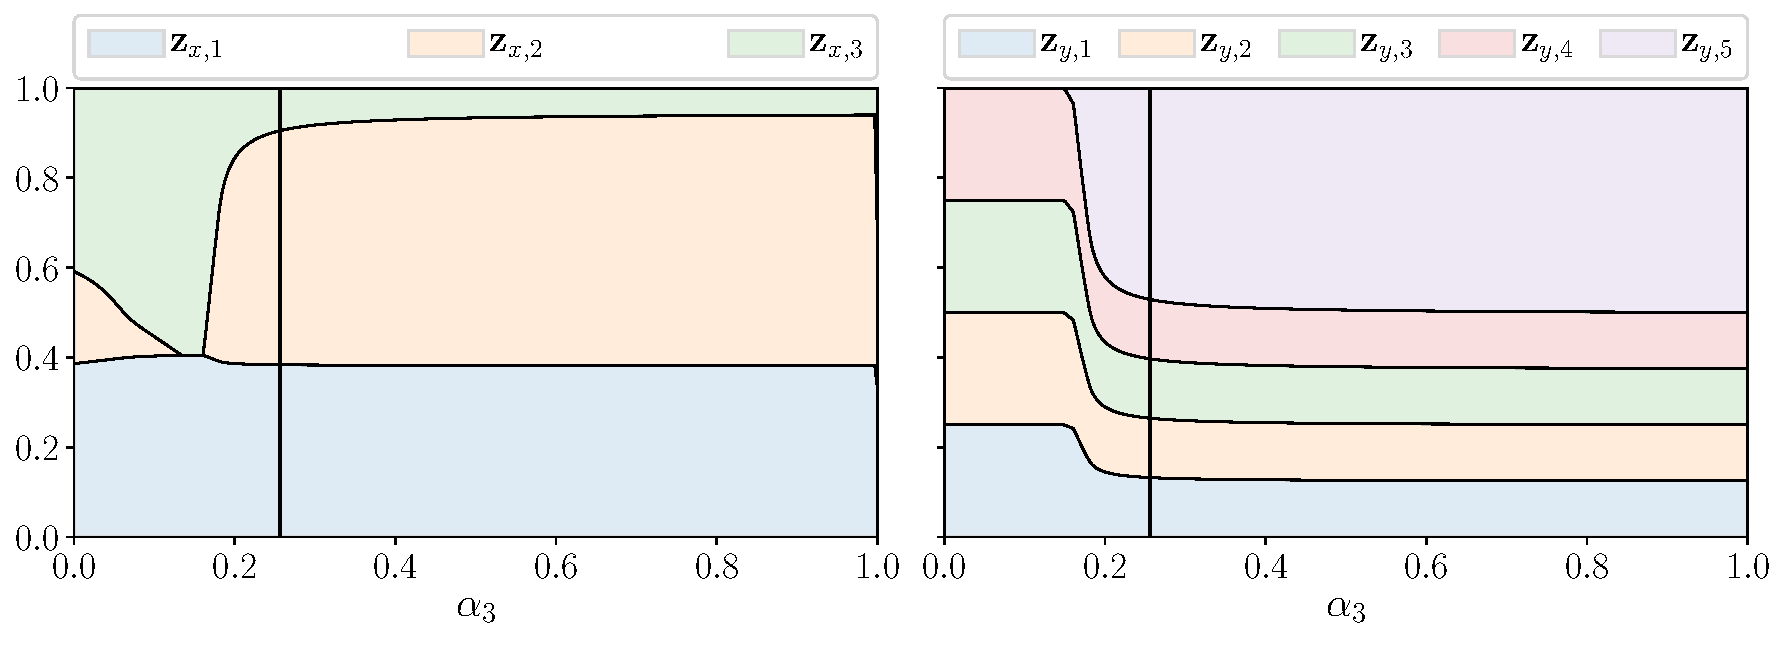
\includegraphics[width=\linewidth]{figs/ch3/features_vs_alpha.pdf}
	\caption{Значимости признаков~$\bz_x$ и целевых векторов~$\bz_y$ в зависимости от~$\alpha_3$ для рассмотренного примера}
	\label{ch3:fig:features_vs_alpha}
\end{figure}

\textbf{Минимаксная постановка задачи выбора признаков.}
Функция~\eqref{ch3:eq:symimp} является симметричной по отношению к~$\bz_x$ и $\bz_y$.
Она штрафует признаки, которые коррелированы и не имеют отношения к целевым векторам.
Кроме того, она штрафует целевые вектора, которые коррелированы между собой и недостаточно коррелируют с признаками.
Это приводит к малым значениям значимостей для целевых векторов, которые слабо коррелируют с признаками, и большим значениям для целевых векторов, которые сильно коррелируют с признаками.
Этот результат противоречит интуиции.
Цель~--- предсказать все целевые вектора, особенно те, которые слабо коррелируют с признаками. Сформулируем две взаимосвязанные задачи:
\begin{align}
	\alpha_1 \cdot \underbrace{\bz_x^{\T} \bQ_x \bz_x}_{\text{Sim}(\bX)} - \alpha_2 \cdot \underbrace{ \bz_x^{\T}\mathbf{B} \bz_y}_{\text{Rel}(\bX, \bY)} \rightarrow \min_{\substack{\bz_x \geq \bZero_n, \\ \bOne_n^{\T}\bz_x=1}},
	\label{ch3:eq:x_qpfs}\\
	\alpha_3 \cdot \underbrace{\bz_y^{\T} \bQ_y \bz_y}_{\text{Sim}(\bY)} + \alpha_2 \cdot \underbrace{ \bz_x^{\T} \mathbf{B} \bz_y}_{\text{Rel}(\bX, \bY)} \rightarrow \min_{\substack{\bz_y \geq \bZero_r,  \\ \bOne_r^{\T}\bz_y=1}}.
	\label{ch3:eq:y_qpfs}
\end{align}
Разница между~\eqref{ch3:eq:x_qpfs} и~\eqref{ch3:eq:y_qpfs} заключается в  знаке перед членом Rel.
В пространстве исходных объектов нерелевантные признаки должны иметь меньшие значения значимости.
В то же время целевые вектора, не релевантные признакам, должны иметь большую значимость.
Задачи~\eqref{ch3:eq:x_qpfs} и \eqref{ch3:eq:y_qpfs} объединяются в совместную минимакс или максмин постановку
\begin{equation}
	\min_{\substack{\bz_x \geq \bZero_n \\ \bOne_n^{\T}\bz_x=1}} 	\max_{\substack{\bz_y \geq \bZero_r \\ \bOne_r^{\T}\bz_y=1}} f(\bz_x, \bz_y), \quad \left(\text {или} \, \max_{\substack{\bz_y \geq \bZero_r \\ \bOne_r^{\T}\bz_y=1}} \min_{\substack{\bz_x \geq \bZero_n \\ \bOne_n^{\T}\bz_x=1}} f(\bz_x, \bz_y)\right),
	\label{ch3:eq:minmax}
\end{equation}
где
\begin{equation*}
	f(\bz_x, \bz_y) = \alpha_1 \cdot \underbrace{\bz_x^{\T} \bQ_x \bz_x}_{\text{Sim}(\bX)} - \alpha_2 \cdot \underbrace{\bz_x^{\T} \bB \bz_y}_{\text{Rel}(\bX, \bY)} - \alpha_3 \cdot \underbrace{\bz_y^{\T} \bQ_y \bz_y}_{\text{Sim}(\bY)}.
\end{equation*}
\begin{theorem}
	Для положительно определенной матрицы~$\bQ_x$ и $\bQ_y$, максмин и минимакс задачи~\eqref{ch3:eq:minmax} имеют одинаковое оптимальное значение.
\end{theorem}
\begin{proof}
	Введём обозначения
	\begin{equation*}
		\mathbb{C}^n = \{\bz : \bz \geq \bZero_n, \, \bOne_n^{\T}\bz=1\}, \quad \mathbb{C}^r = \{\bz : \bz \geq \bZero_r, \, \bOne_r^{\T}\bz=1\}.
	\end{equation*}
	Множества $\mathbb{C}^n$ и $\mathbb{C}^r$ компактные и выпуклые. Функция $f: \mathbb{C}^n \times \mathbb{C}^r \rightarrow \bbR$ является непрерывной. Если~$\bQ_x$ и $\bQ_y$ положительно определенны, функция~$f$ является выпукло-вогнутой. Таким образом
	$f(\cdot, \bz_y): \mathbb{C}^n \rightarrow \bbR$ выпуклая при фиксированном~$\bz_y$, а $f(\bz_x, \cdot): \mathbb{C}^r \rightarrow \bbR$ вогнута при фиксированном~$\bz_x$.
	В этом случае по теореме Неймана о минимаксе
	\begin{equation*}
		\min_{\bz_x \in \mathbb{C}^n} \max_{\bz_y \in \mathbb{C}^r} f(\bz_x, \bz_y) = \max_{\bz_y \in \mathbb{C}^r} \min_{\bz_x\in \mathbb{C}^n} f(\bz_x, \bz_y).
	\end{equation*}
\end{proof}

Для решения минимакс задачи~\eqref{ch3:eq:minmax}, зафиксируем некоторый~$\bz_x \in \mathbb{C}^n$. Для фиксированного вектора~$\bz_x$ решаем задачу
\begin{equation}
	\max_{\bz_y \in \mathbb{C}_r} f(\bz_x, \bz_y) = \max_{\substack{\bz_y \geq \bZero_r \\ \bOne_r^{\T}\bz_y=1}} \bigl[\alpha_1 \cdot \bz_x^{\T} \bQ_x \bz_x - \alpha_2 \cdot \bz_x^{\T} \bB \bz_y - \alpha_3 \cdot \bz_y^{\T} \bQ_y \bz_y \bigr].
	\label{ch3:eq:fixed_ax}
\end{equation}
Лагранжиан для данной задачи:
\begin{equation*}
	L(\bz_x, \bz_y, \lambda, \bmu) = \alpha_1 \cdot \bz_x^{\T} \bQ_x \bz_x - \alpha_2 \cdot \bz_x^{\T} \bB \bz_y - \alpha_3 \cdot \bz_y^{\T} \bQ_y \bz_y + \lambda \cdot  (\bOne_r^{\T} \bz_y - 1) + \bmu^{\T} \bz_y.
\end{equation*}
Здесь вектор множителей Лагранжа~$\bmu$, который соответствует ограничениям на неравенства $\bz_y \geq \bZero_r$, является неотрицательным.
Двойственной задачей является
\begin{equation}
	\min_{\lambda, \, \bmu \geq \bZero_r} g(\bz_x, \lambda, \bmu) = \min_{\lambda, \, \bmu \geq \bZero_r}  \left[\max_{\bz_y \in \bbR^r} L(\bz_x, \bz_y, \lambda, \bmu) \right].
	\label{ch3:eq:dual}
\end{equation}
Для задачи квадратичного программирования~\eqref{ch3:eq:fixed_ax} с положительно определенными матрицами~$\bQ_x$ и~$\bQ_y$ выполняются условия сильной двойственности. Таким образом, оптимальное значение~\eqref{ch3:eq:fixed_ax} равно оптимальному значению~\eqref{ch3:eq:dual}. Это позволяет перейти от решения задачи~\eqref{ch3:eq:minmax} к решению задачи
\begin{equation}
\min_{\bz_x \in \mathbb{C}^n, \, \lambda, \, \bmu \geq \bZero_r} g(\bz_y, \lambda, \bmu).
\label{ch3:eq:dual_maxmin}
\end{equation}

Полагая градиент~$\nabla_{\bz_y} L(\bz_x, \bz_y, \lambda, \bmu)$ равным нулю, получим оптимальное значение~$\bz_y$:
\begin{equation*}
	\bz_y = \frac{1}{2\alpha_3} \bQ_y^{-1} \left( - \alpha_2 \cdot \bB^{\T} \bz_x +\lambda \cdot \bOne_r + \bmu \right).
\end{equation*}
Двойственная функция принимает вид
\begin{multline}
	g(\bz_x, \lambda, \bmu)
	= \max_{\bz_y \in \bbR^r} L(\bz_x, \bz_y, \lambda, \bmu) =
	\bz_x^{\T} \left( - \frac{\alpha_2^2}{4\alpha_3} \cdot \bB \bQ_y^{-1} \bB^{\T} - \alpha_1 \cdot \bQ_x\right) \bz_x \\ - \frac{1}{4 \alpha_3} \lambda^2 \cdot \bOne_r^{\T} \bQ_y^{-1} \bOne_r - \frac{1}{4 \alpha_3} \cdot \bmu^{\T} \bQ_y^{-1} \bmu + \frac{\alpha_2}{2 \alpha_3} \lambda \cdot \bOne_r^{\T} \bQ_y^{-1} \bB^{\T} \bz_x \\ - \frac{1}{2 \alpha_3} \lambda \cdot \bOne_r^{\T} \bQ_y^{-1} \bmu + \frac{\alpha_2}{2 \alpha_3} \cdot \bmu^{\T} \bQ_y^{-1} \bB^{\T} \bz_x + \lambda.
	\label{ch3:eq:dual_quadratic_form}
\end{multline}
Тем самым задача~\eqref{ch3:eq:dual_maxmin} является квадратичной задачей с~$n + r + 1$ переменными.

\textbf{Несимметричный учёт значимостей признаков и целевых переменных.}
Естественным способом преодоления проблемы метода SymImp является добавление штрафа для целевых векторов, которые коррелируют с признаками.
Добавим линейный член~$\bb^{\T} \bz_y$ в член $\text{Rel}(\bX, \bY)$ следующим образом:
\begin{equation}
	\alpha_1 \cdot \underbrace{\bz_x^{\T} \bQ_x \bz_x}_{\text{Sim}(\bX)} - \alpha_2 \cdot  \underbrace{\left(\bz_x^{\T} \bB \bz_y - \bb^{\T} \bz_y \right) }_{\text{Rel}(\bX, \bY)} + \alpha_3 \cdot \underbrace{\bz_y^{\T} \bQ_y \bz_y}_{\text{Sim}(\bY)} \rightarrow \min_{\substack{\bz_x \geq \bZero_n, \, \bOne_n^{\T}\bz_x=1 \\ \bz_y \geq \bZero_r, \, \bOne_r^{\T}\bz_y=1}}.
	\label{ch3:eq:asymimp}
\end{equation}
\begin{statement}
	Пусть вектор $\bb$ равен
	\begin{equation*}
	b_j = \max_{i=1, \dots n} [\bB]_{i, j}.
	\end{equation*}
	Тогда значение коэффициентов значимостей вектора~$\bz_y$ будут неотрицательными в~$\text{Rel}(\bX, \bY)$ для задачи~\eqref{ch3:eq:asymimp}.
\end{statement}
\begin{proof}
	Утверждение следует из факта
	\[
	\sum_{i=1}^n  z_i b_{ij} \leq \left(\sum_{i=1}^n z_i \right)\max_{i=1, \dots n} b_{ij} = \max_{i=1, \dots n} b_{ij},
	\]
	где $z_i \geq 0$ и $\sum_{i=1}^n z_i = 1$.
\end{proof}
Следовательно, функция~\eqref{ch3:eq:asymimp} штрафует в меньшей мере признаки, которые имеют отношение к целевым векторам, и целевые вектора, которые недостаточно коррелированы с признаками.
\begin{statement}
	Баланс между членами~$\text{Sim}(\bX)$, $\text{Rel}(\bX, \bY)$ и $\text{Rel}(\bX, \bY)$ для задачи~\eqref{ch3:eq:asymimp} достигается при следующих коэффициентах:
	\begin{equation*}
		\alpha_1 \propto \overline{\bQ}_y \left( \overline{\bb} - \overline{\bB}\right), \quad
		\alpha_2 \propto \overline{\bQ}_x \overline{\bQ}_y, \quad
		\alpha_3  \propto \overline{\bQ}_x \overline{\bB}.
	\end{equation*}
\end{statement}
\begin{proof}
	Необходимые значения~$\alpha_1$, $\alpha_2$, и $\alpha_3$ являются решением следующей системы уравнений:
	\begin{align}
		&\alpha_1 + \alpha_2 + \alpha_3 = 1, \\
		&\alpha_1 \overline{\bQ}_x = \alpha_2 \overline{\bB}, \label{ch3:eq:asymimp_balance1}\\
		&\alpha_2 \left(\overline{\bb} - \overline{\bB} \right) = \alpha_3 \overline{\bQ}_y.
		\label{ch3:eq:asymimp_balance2}
	\end{align}
	Здесь, в~\eqref{ch3:eq:asymimp_balance1} уравновешены $\text{Sim}(\bX)$ с первым слагаемым~$\text{Rel}(\bX, \bY)$, а в~\eqref{ch3:eq:asymimp_balance2} уравновешены $\text{Sim}(\bY)$  с~$\text{Rel}(\bX, \bY)$.
\end{proof}
\begin{statement}
	Для случая $r=1$, предложенные функции~\eqref{ch3:eq:symimp},~\eqref{ch3:eq:minmax} и~\eqref{ch3:eq:asymimp} совпадают с оригинальным методом QPFS~\eqref{ch3:eq:qpfs_problem}.
	
	\begin{proof}
		Если $r$ равно 1, то $\bQ_y = q_y$~--- скаляр, $\bz_y = 1$ и $\bB = \bb$. Задачи~\eqref{ch3:eq:symimp},~\eqref{ch3:eq:minmax} и~\eqref{ch3:eq:asymimp} принимают вид
		\begin{equation*}
		\alpha_1 \cdot \bz_x^{\T} \bQ_x \bz_x - \alpha_2 \cdot \bz_x^{\T} \bb \rightarrow \min_{\bz_x \geq \bZero_n, \, \bOne_n^{\T}\bz_x=1} .
		\end{equation*}
		При $\alpha = \frac{\alpha_2}{\alpha_1 + \alpha_2}$ последняя задачи принимает вид~\eqref{ch3:eq:qpfs_problem}.
	\end{proof}
\end{statement}

Таблица~\ref{ch3:tbl:summary} демонстрирует основные идеи и функции ошибок для каждого метода. 
RelAgg является базовой стратегией и не учитывает корреляции в целевом пространстве.
SymImp штрафует попарные корреляции между целевыми векторами.
MinMax более чувствителен к целевым векторам, которые трудно предсказать.
Стратегия Asymimp добавляет линейный член к функции SymImp, чтобы сделать вклад признаков и целевых векторов асимметричным.

\begin{table}[ht]
	\centering
	\caption{Обзор предлагаемых обобщений метода QPFS для векторной целевой переменной}
	\small{
		\begin{tabular}{c|c|c}
			\hline
			Метод & Идея & Функция ошибки $S(\bz | \bX, \bY)$ \\
			\hline && \\ [-.5em]
			RelAgg & $\min \bigl[ \text{Sim}(\bX) - \text{Rel}(\bX, \bY) \bigr] $ & $\min\limits_{\bz_x} \bigl[ (1 - \alpha) \cdot \bz_x^{\T} \bQ_x \bz_x - \alpha \cdot \bz_x^{\T} \bB \bOne_r \bigr] $ \\ &&\\[-.5em]
			SymImp & $\begin{aligned} \min \, \bigl[ \text{Sim}(\bX) & - \text{Rel}(\bX, \bY) \\ & + \text{Sim}(\bY) \bigr] \end{aligned}$ & $ \min\limits_{\bz_x, \, \bz_y} \left[ \alpha_1 \cdot \bz_x^{\T} \bQ_x \bz_x - \alpha_2 \cdot \bz_x^{\T} \bB \bz_y + \alpha_3 \cdot \bz_y^{\T} \bQ_y \bz_y \right] $\\ &&\\ [-.5em]
			MinMax & $\begin{aligned} &\min \, \bigl[ \text{Sim}(\bX) - \text{Rel}(\bX, \bY) \bigr]  \\ & \max \bigl[\text{Rel}(\bX, \bY) + \text{Sim}(\bY) \bigr] \end{aligned}$ & $	\min\limits_{\bz_x} 	\max\limits_{\bz_y} \bigl[\alpha_1 \cdot \bz_x^{\T} \bQ_x \bz_x - \alpha_2 \cdot \bz_x^{\T} \bB \bz_y - \alpha_3 \cdot \bz_y^{\T} \bQ_y \bz_y \bigr]$ \\ &&\\ [-.5em]
			AsymImp & $\begin{aligned} & \min \, \bigl[ \text{Sim}(\bX) - \text{Rel}(\bX, \bY) \bigr]\\ &  \max \bigl[\text{Rel}(\bX, \bY) + \text{Sim}(\bY) \bigr] \end{aligned}$ & $\min\limits_{\bz_x, \bz_y} \bigl[ \alpha_1 \cdot \bz_x^{\T} \bQ_x \bz_x - \alpha_2 \cdot \left(\bz_x^{\T} \bB \bz_y - \bb^{\T} \bz_y \right) + \alpha_3 \cdot \bz_y^{\T} \bQ_y \bz_y \bigr]$\\ 
			\hline
	\end{tabular}}
	\label{ch3:tbl:summary}
\end{table}


%%%%%%%%%%%%%%%%%%%%%%%%%%%%%%%%%%%%%%%%%%%%%%%%
\section{Анализ методов учета значимостей целевых переменных}
\label{sec:ch3:exp_mqpfs}
%%%%%%%%%%%%%%%%%%%%%%%%%%%%%%%%%%%%%%%%%%%%%%%%

\textbf{Внешние критерии качества.} Для оценки предложенных методов выбора признаков, введём критерии оценки качества выбранного подмножества признаков.
Определим коэффициент мультикорреляции как среднее значение коэффициента множественной корреляции следующим образом:
\begin{equation*}
R^2 = \frac{1}{r} \text{tr} \left( \bC^{\T} \mathbf{R}^{-1} \bC \right), \quad \text{где }\bC = [ \text{corr}(\bchi_i, \bnu_j)]_{\substack{i=1, \dots, n \\ j=1, \dots, r}}, \,\, \mathbf{R} = [ \text{corr}(\bchi_i, \bchi_j)]_{i, j = 1}^n.
\end{equation*}
Этот коэффициент принимает значение между 0 и 1. Большее значение~$R^2$ соответствует лучшему подмножеству признаков.

Нормированная среднеквадратичная ошибка (sRMSE) отображает качество прогнозирования модели. Оценка sRMSE считается на тренировочной и тестовой выборке.
\begin{equation*}
\text{sRMSE}(\bY, \widehat{\bY}_{\ba}) = \sqrt{\frac{\text{MSE} (\bY, \widehat{\bY}_{\ba})}{\text{MSE} (\bY, \overline{\bY})}} =  \frac{\| \bY - \widehat{\bY}_{\ba} \|_2}{\| \bY - \overline{\bY} \|_2}.
\end{equation*}
Здесь $\widehat{\bY}_{\ba} = \bX_{\ba} \bTheta_{\ba}^{\T}$~--- прогноз модели, $\overline{\bY}$~--- предсказание константной модели, полученное усреднением целевой переменной по всем объектам.
Данный показатель на тестовой выборке необходимо минимизировать.

Байесовский информационный критерий (BIC)~--- компромисс между качеством предсказания и размером выбранного подмножества признаков~$\|\ba\|_0 = \#\{j: a_j \neq 0\}= \sum_{j=1}^n a_j$:
\begin{equation*}
\text{BIC} = m \ln \left( \text{MSE} ( \bY, \widehat{\bY}_{\ba})\right) + \| \ba \|_0 \cdot \ln m.
\end{equation*}
Чем меньше значение BIC, тем лучше набор признаков.

\textbf{Данные.}
Вычислительный эксперимент проводился на данных электрокортикограмм. Описание данных приведено в разделе~\ref{sec:ch2:exp_linear}.

На Рис.~\ref{ch3:fig:corr_matrix} показаны матрицы корреляций для исходных матриц~$\bX$ и~$\bY$ данных ECoG. Частоты в матрице~$\bX$ сильно коррелированы. 
В целевой матрице~$\bY$ корреляции между осями несущественны по сравнению с корреляциями между последовательными моментами времени и эти корреляции спадают со временем.
\begin{figure}[ht]
	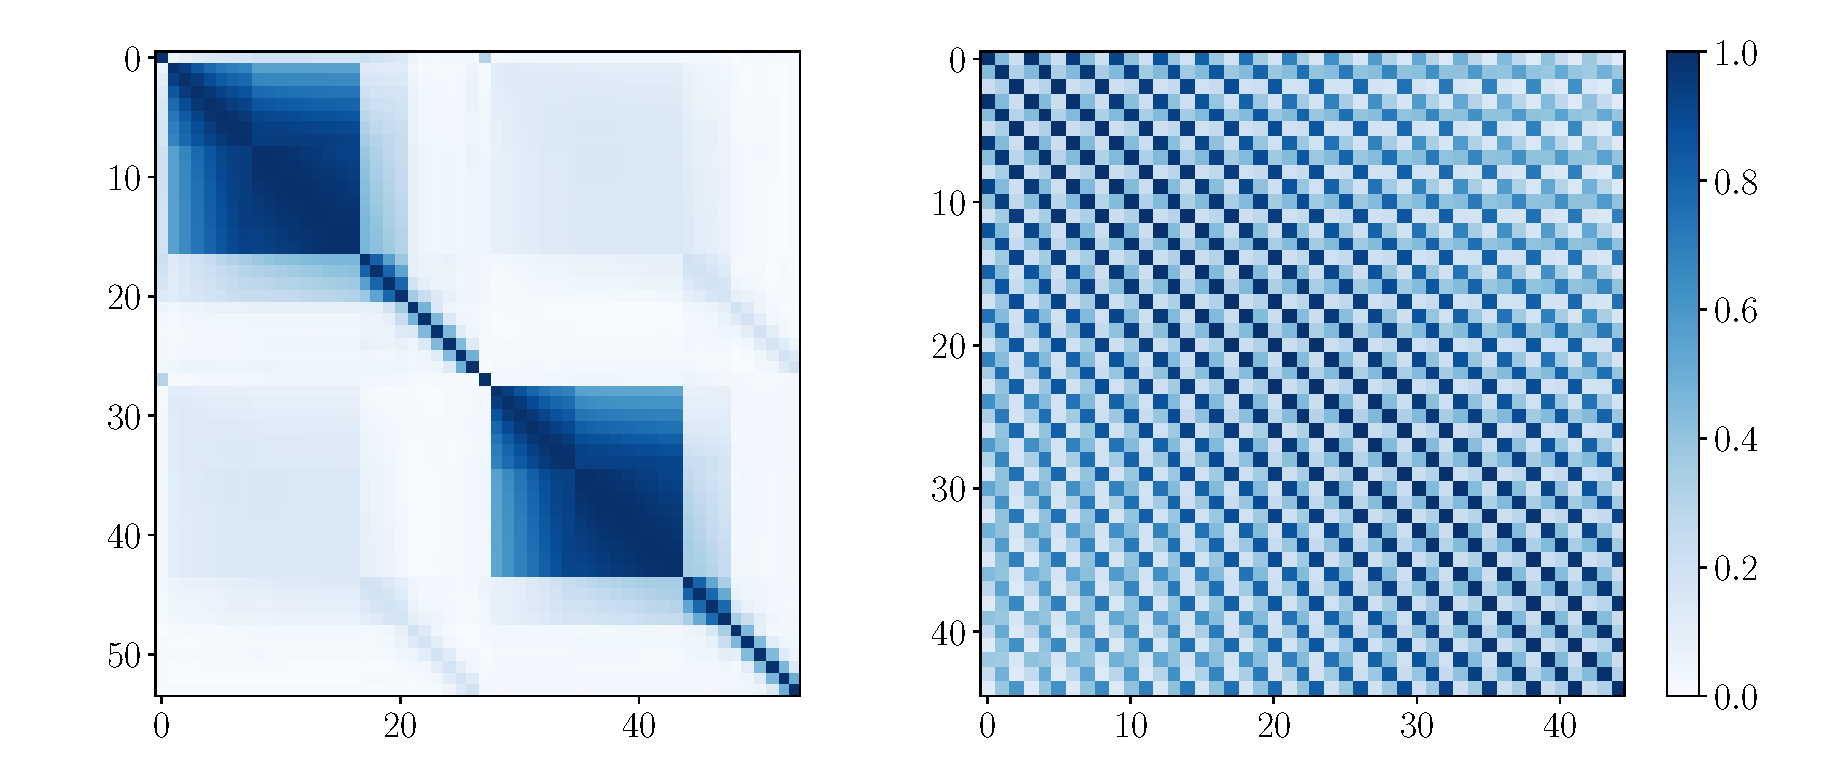
\includegraphics[width=\linewidth]{figs/ch3/corr_matrix}
	\caption{Матрицы корреляций для матрицы плана~$\bX$ и целевой матрицы~$\bY$ для данных ECoG}
	\label{ch3:fig:corr_matrix}
\end{figure}

\textbf{Результаты.}
Применим метод SymImp QPFS для различных значений коэффициента~$\alpha_3$ согласно формуле~\eqref{ch3:eq:alphas3}.
Зависимость значимостей целевых векторов~$\bz_y$ относительно коэффициента~$\alpha_3$ для различных значений~$k$ показана на Рис.~\ref{ch3:fig:features_vs_alpha_ecog}.
Значимости целевых векторов почти одинаковы для всех координат запястья при прогнозировании одного отсчёта времени ($k = 1$), 
что отражает независимость между координатами $x$, $y$ и $z$.
Для $k = 2$ и $k = 3$ значимости некоторых целевых векторов становятся нулевыми при увеличении~$\alpha_3$.
Вертикальные линии соответствуют оптимальному значению~$\alpha_3$, вычисленному по~\eqref{ch3:eq:alpha_3}. 
При этом значении $\alpha_3$ значимости компонент~$\bz_y$ совпадают. 
Таким образом, метод не учитывает различия между целевыми векторами для $k=1, 2, 3$.

\begin{figure}[ht]
	\begin{minipage}{.5\linewidth}
		\subfloat{
			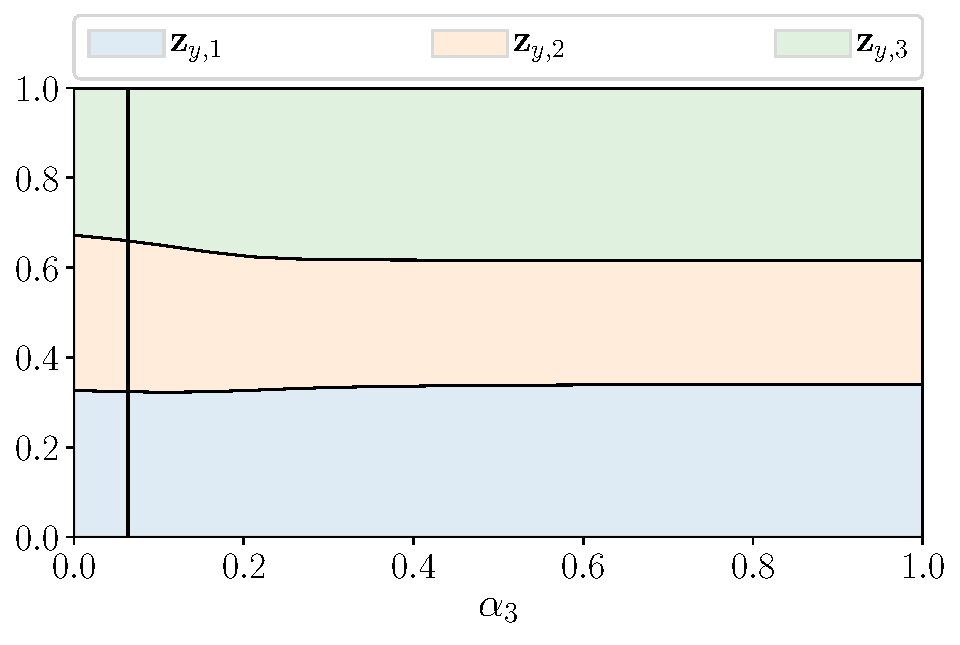
\includegraphics[width=\linewidth]{figs/ch3/features_vs_alpha_ecog_3}}
	\end{minipage}%
	\begin{minipage}{.5\linewidth}
		\subfloat{
			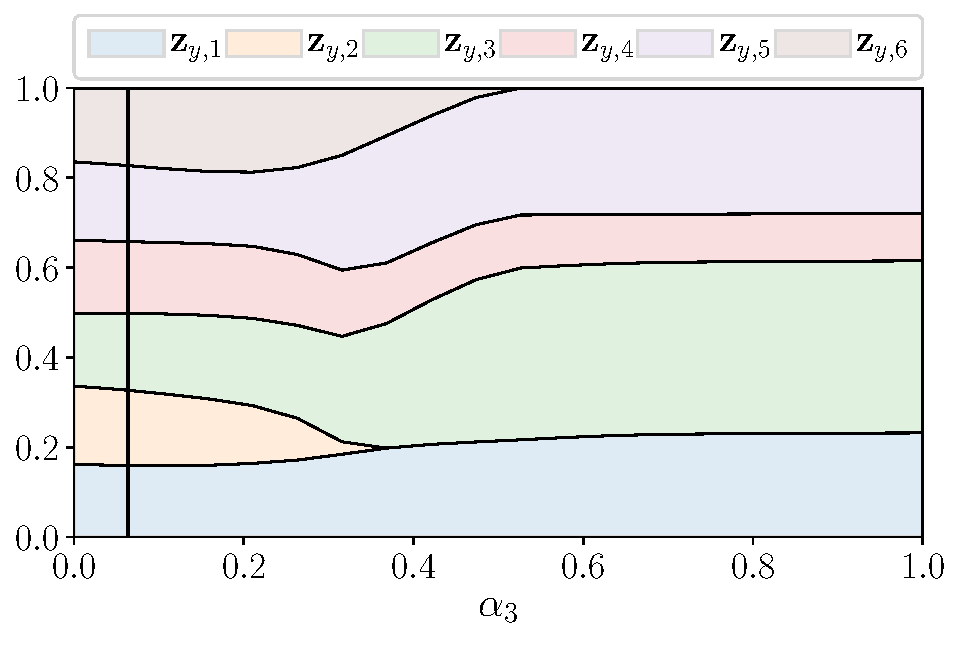
\includegraphics[width=\linewidth]{figs/ch3/features_vs_alpha_ecog_6}}
	\end{minipage}\par\medskip
	\subfloat{
		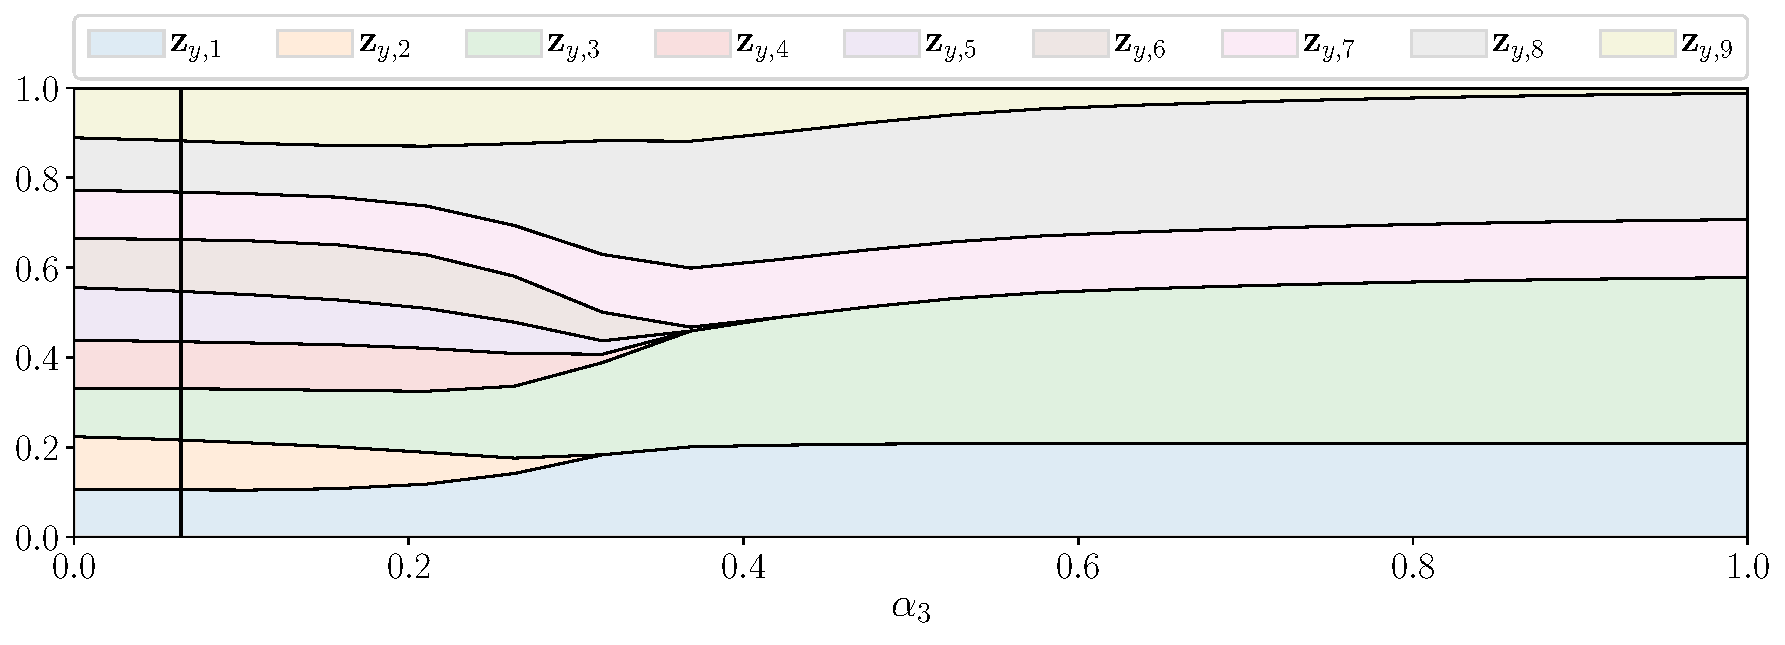
\includegraphics[width=\linewidth]{figs/ch3/features_vs_alpha_ecog_9}}
	
	\caption{Значимости целевых векторов~$\bz_y$ в зависимости от~$\alpha_3$ для метода SymImp QPFS}
	\label{ch3:fig:features_vs_alpha_ecog}
\end{figure}

Предлагаемые методы QPFS для случая векторной целевой переменной, приведенные в таблице~\ref{ch3:tbl:summary} применяются для набора данных ECoG. 
Решим задачу выбора признаков для каждого из методов, чтобы получить вектора значимостей признаков. 
Отсортируем по убыванию признаки по значению их значимостей. Обучим линейную модель, постепенно добавляя в неё признаки. 
Исследуются значения описанных критериев качества при увеличении количества отобранных признаков. 
На Рис.~\ref{ch3:fig:ecog_3_30_metrics} показаны результаты для случая прогнозирования $k = 30$ отсчётов времени. 
Порог значимости признаков~$\tau$ обозначен цветными тиками. 
Пороговые значения $\tau$ для предлагаемых методов больше, чем для базового метода RelAgg. 
Метод SymImp имеет большой порог, не позволяя получить малый набор признаков.
Однако метод SymImp обладает наилучшей предсказательной способностью с точки зрения sRMSE на тестовых данных.
Второй по качеству результат по sRMSE показал метод AsymImp.
Все предложенные методы достигают меньшей ошибки на тестовой выборке по сравнению с методом RelAgg. 
Критерий устойчивости также выше для предложенных методов.
Метод AsymImp показывает лучшие результаты с точки зрения качества прогнозирования и размера выбранного подмножества признаков.

\begin{figure}[ht]
	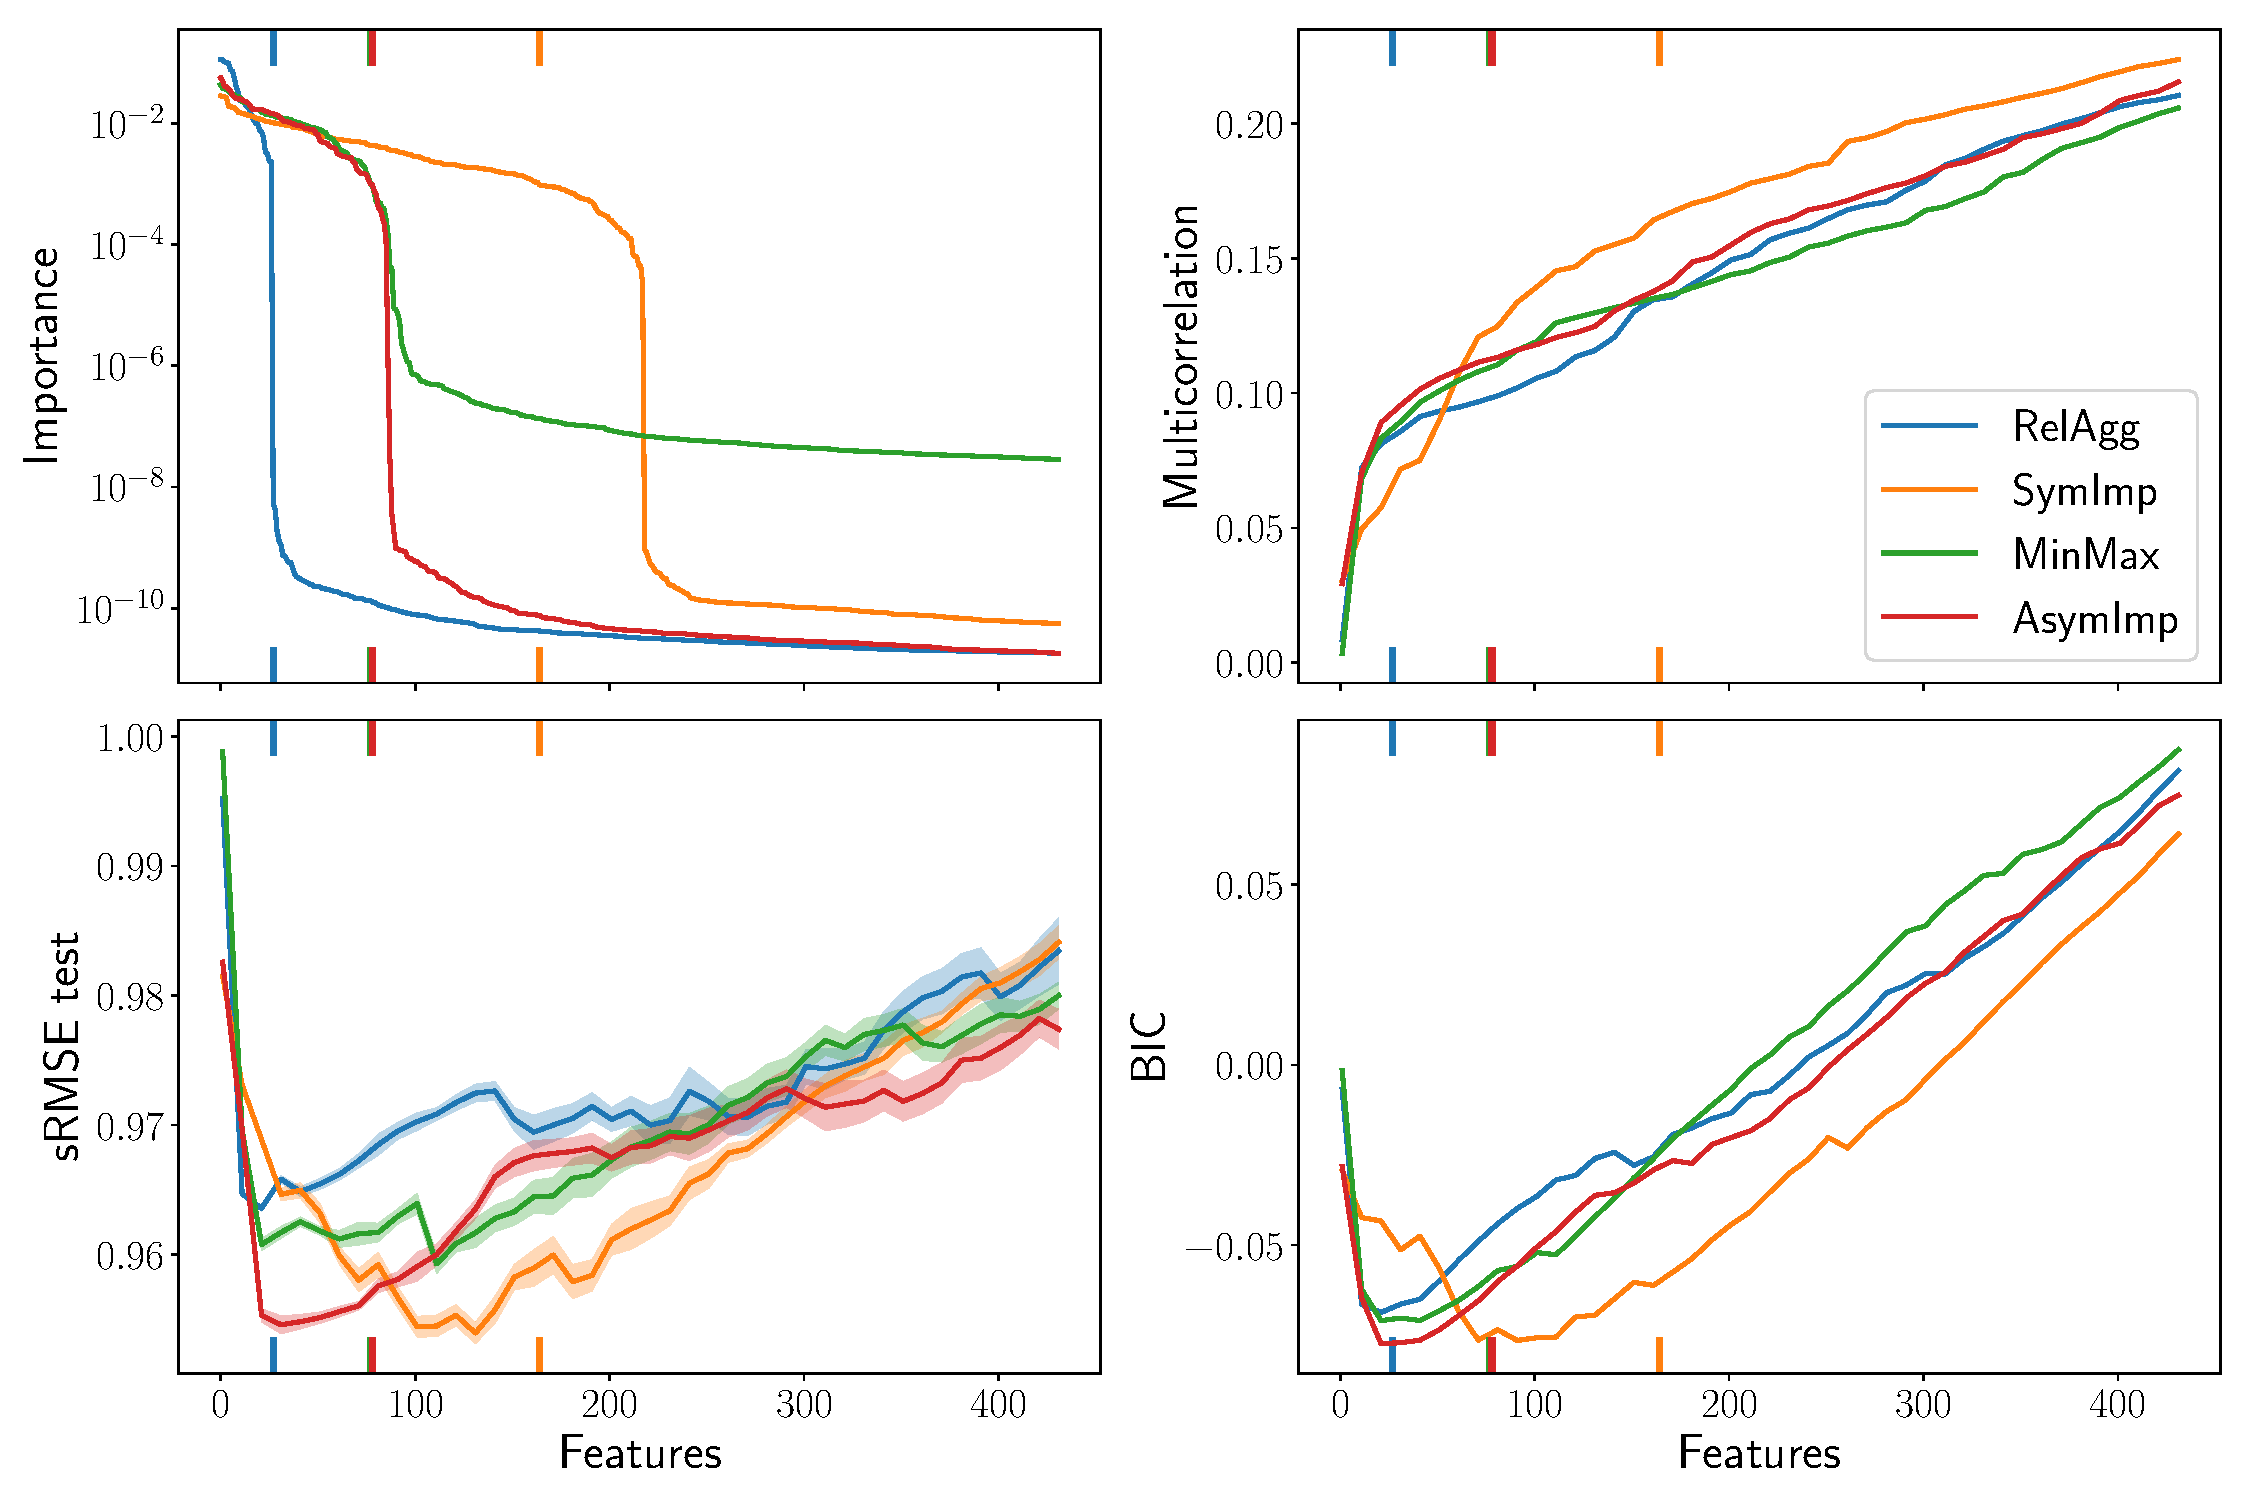
\includegraphics[width=\linewidth]{figs/ch3/ecog_3_30_metrics}
	\caption{Сравнение предложенных методов выбора признаков для данных ECoG при прогнозировании $k = 30$ отсчётов времени}
	\label{ch3:fig:ecog_3_30_metrics}
\end{figure}

Чтобы сравнить структуру выбранных подмножеств признаков и исследовать стабильность процедуры выбора признаков, используется метод генерации данных с помощью бутстрепа. 
Генерируется множество подвыборок, выбирая объекты по одному с возвращениями. 
Затем решается задача выбора признаков для каждой пары матрицы исходных объектов~$\bX$ и  матрицы целевых объектов~$\bY$.
Сравниваются полученные вектора значимостей для различных подвыборок данных. 
В качестве меры стабильности работы методов вычисляется средний попарный коэффициент корреляции Спирмена и попарное $\ell_2$ расстояние.
В таблице~\ref{ch3:tbl:stability} показана средняя ошибка sRMSE, размер подмножества признаков и описанные статистики для каждого метода. 
Ошибка считалась на обученной линейной модели с использованием $50$ признаков с наибольшими значениями значимостей.
Asymimp дает наименьшую ошибку на тестовой выборке. 
Размер выбранных подмножеств объектов завышен при использовании порогового значения~$\tau=10^{-4}$. 
Оптимальное значение~$\tau$ может быть подобрано с помощью процедуры кросс-валидации.

\begin{table}[ht]
	\caption{Стабильность предложенных методов выбора признаков}
	\centering
	\begin{tabular}{l|ccccc}
		\hline
		& sRMSE  & $\|\ba\|_0$ & Spearman $\rho$ & $\ell_2$ \\ \hline
		RelAgg & 0.965 $\pm$ 0.002 & 26.8 $\pm$ 3.8 & 0.915 $\pm$ 0.016 & 0.145 $\pm$ 0.018   \\
		SymImp & 0.961 $\pm$ 0.001 & 224.4 $\pm$ 9.0 & 0.910 $\pm$ 0.017 & 0.025 $\pm$ 0.002   \\
		MinMax & 0.961 $\pm$ 0.002 & 101.0 $\pm$ 2.1& 0.932 $\pm$ 0.009 & 0.059 $\pm$ 0.004   \\
		AsymImp & 0.955 $\pm$ 0.001 & 85.8 $\pm$ 10.2& 0.926 $\pm$ 0.011 & 0.078 $\pm$ 0.007  \\ \hline
	\end{tabular}
	\label{ch3:tbl:stability}
\end{table}

Для того, чтобы сравнить методы снижения размерности и выбора признаков, используется модель PLS, описанная в главе~\ref{ch:pls}. 
На Рис.~\ref{ch3:fig:pls_vs_k} показана ошибка sRMSE на тренировочной и тестовой выборках в зависимости от размерности скрытого пространства~$l$.
Ошибка на тестовой выборке достигает минимума при $l = 11$.
Метод PLS является более гибким подходом по сравнению с линейной моделью, построенной на подмножестве признаков, так как использует все исходные признаки.
Это приводит к меньшей ошибке, но модель не является разреженной.

На Рис.~\ref{ch3:fig:models} приведено сравнение 3 моделей: линейной регрессии; регрессии PLS, построенной на 100 признаках QPFS; регрессии PLS со всеми признаками.
Линейная регрессия со всеми признаками не рассматривается, так как ее результаты близки к константному прогнозу. На рисунке также приведены результаты методов lasso и elastic net, которые широко используются для выбора признаков.
В данном эксперименте использовался метод Asymimp QPFS.
Размерность скрытого пространства PLS $l = 15$.
Результаты регрессии PLS значительно лучше, линейной регрессии с признаками QPFS.
Это означает, что последняя модель не является достаточно гибкой.
Тем не менее, лучший результат показывает модель PLS, построенная на признаках QPFS. 
Данная модель является разреженной, так как использует только 100 исходных признаков.
Способность модели PLS находить оптимальное скрытое представление данных улучшает предсказательную способность модели.

\begin{figure}[ht]
	\begin{minipage}{.41\linewidth}
		\centering
		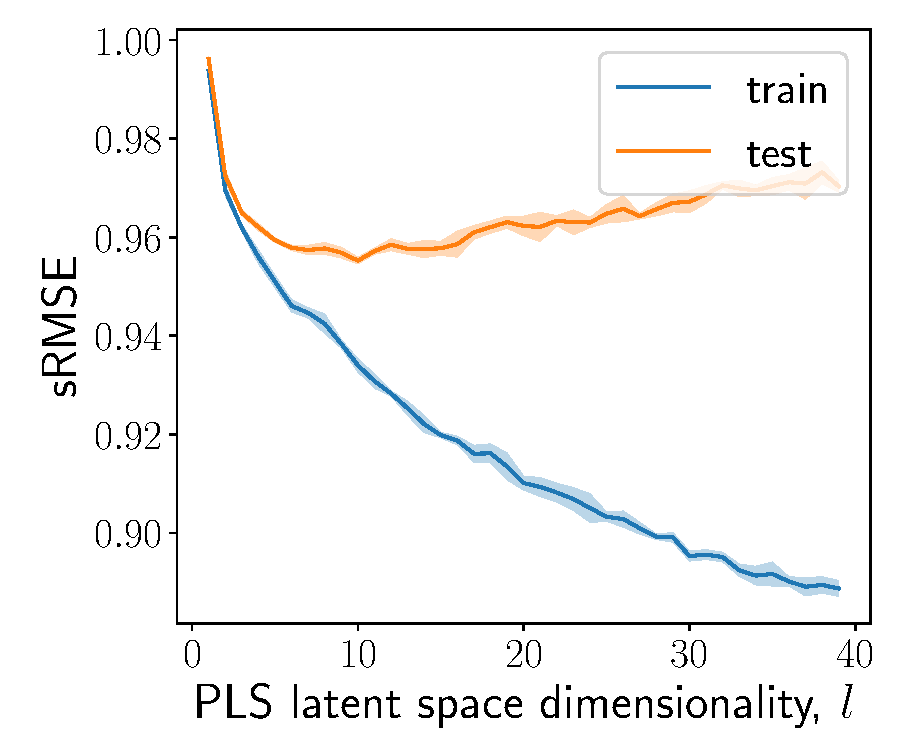
\includegraphics[width=1.\linewidth]{figs/ch3/pls_vs_k}
		\caption{ Ошибка sRMSE на тестовой выборке для модели PLS}
		\label{ch3:fig:pls_vs_k}
	\end{minipage}%
	\begin{minipage}{.55\linewidth}
		\centering
		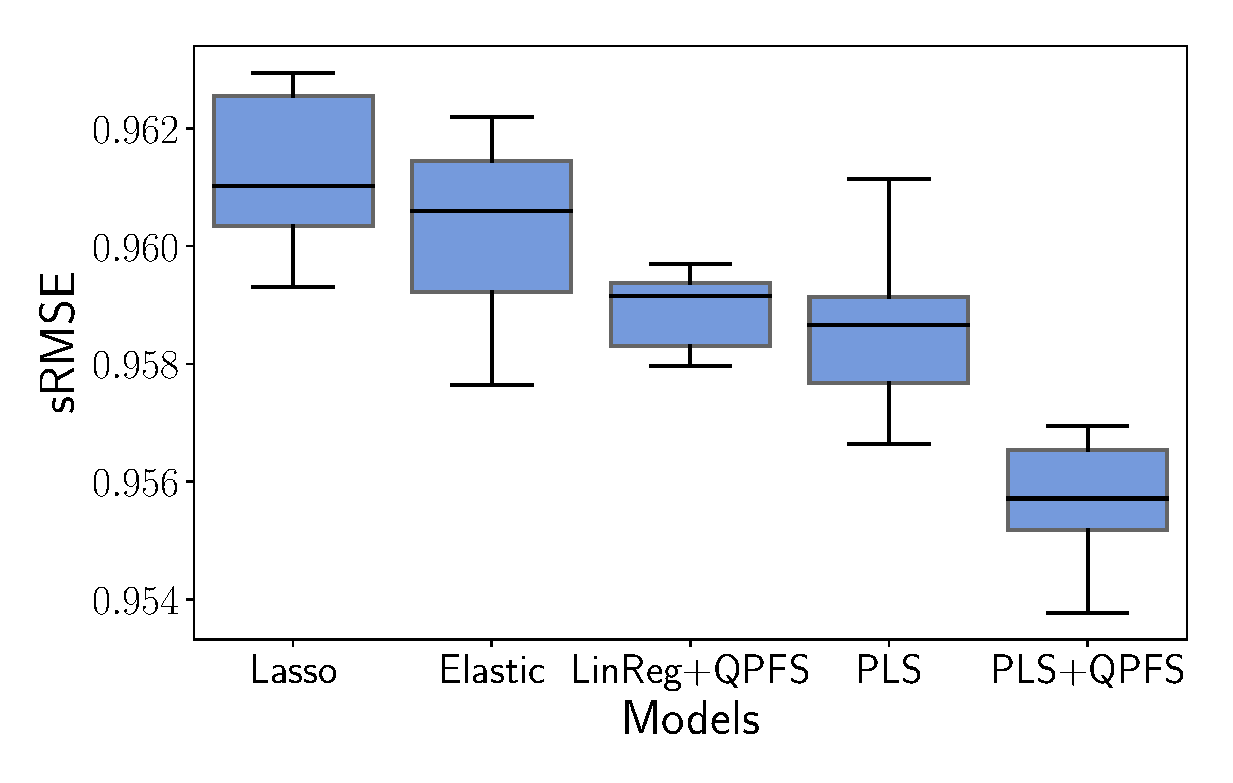
\includegraphics[width=1.\linewidth]{figs/ch3/models2}
		\caption{Диаграммы размаха значений sRMSE на тестовой выборке для моделей Lasso, Elastic, LinReg+QPFS, PLS, PLS+QPFS}
		\label{ch3:fig:models}
	\end{minipage}
\end{figure}
